\section{Wykorzystane technologie}
  \subsection{Ruby}
  Ruby jest w pełni obiektowym, wysokopoziomowym językiem programowania. Jego twórca, Yukihiro “Matz” Matsumoto, chciał stworzyć język jeszcze bardziej obiektowy niż Python, dlatego każdy fragment informacji może uzyskać swoje właściwości i metody. Autor czerpał inspiracje ze swoich ulubionych języków: Perla, Smalltalka, Eiffel, Ady i Lispa. Po za obiektowością, Rubiego cechuje też prosta składnia, ułożona w sposób umożliwiający pisanie prostego i czytelnego kodu. Ponadto, jest to język niezwykle elastyczny, ponieważ pozwala użytkownikom dowolnie modyfikować jego składowe. Programista może dopisać, rozszerzyć jakiś moduł, lub usunąć z niego jakąś część. Powstał w 1995 roku, lecz dopiero w 2005 roku zyskał na popularności za sprawą frameworka Ruby on Rails, który został w nim napisany. Dzisiaj osoby piszące w Rubym to jedni z najlepiej zarabiających programistów w USA\footnote{\url{http://www.pb.pl/3945225,84037,te-jezyki-programowania-daja-najlepiej-zarobic-w-usa}}.

  \subsection{Ruby on Rails}
  Jest to framework, platforma programistyczna, pozwalająca na szybkie tworzenie stron i aplikacji internetowych. Została napisana przez duńskiego programistę Davida Heinemeiera Hanssona, zwanego potocznie DHH. Oparta jest o wzorzec projektowy MVC\footnote{Model View Controller, więcej informacji w rozdziale poświęconym wykorzystanym wzorcom projektowym w pracy.}. \\
  Tim O'Reilly, założyciel O'Reilly Media, powiedział:
  \begin{quote}
    \emph{“Ruby on Rails jest przełomem w dziedzinie programowania aplikacji internetowych.
    Potężne aplikacje, których tworzenie do tej pory zabierało tygodnie czy miesiące, są teraz tworzone dosłownie w kilka dni.”}
  \end{quote}
  W Ruby on Rails panuje zasada \emph{Convention over configuration}, konwencja ponad konfiguracją, co znaczy, że nie trzeba się przejmować skomplikowanymi plikami konfiguracyjnymi, tylko wystarczy postępować według przyjętych przez twórców schematów. Railsy mają wbudowany serwer lokalny, co pozwala na szybkie testowanie aplikacji, bez zbędnego i czasochłonnego umieszczania kodu na zewntęrznej maszynie.

  \subsection{Git}
  To rozproszony system kontroli wersji, bardzo pomocny w projektach, przy których pracuje kilka osób. Ale nie tylko. Programiści pracujący w pojedynke, też bardzo często korzystają z takiego oprogramowania, ponieważ widać wszystkie zmiany wcześniej wprowadzane i w łatwy sposób można wrócić do wcześniejszych wersji. Użytkownik posługuję się tzw. commitami. Jest to nic innego jak zatwierdzenie zmian w plikach. Podobny narzędziem do Gita jest SVN. Różnica między nimi polega na tym, że Git kopiuje całe repozytorium na komputer, programista zatwierdza zmiany lokalnie i dopiero na koniec wrzuca je na serwer. W przypadku SVN całość trzymana jest na serwerze. Różnice między tymi dwoma technologiami pokazuje poniższy obrazek.

  \begin{figure}[h]
    \centering
    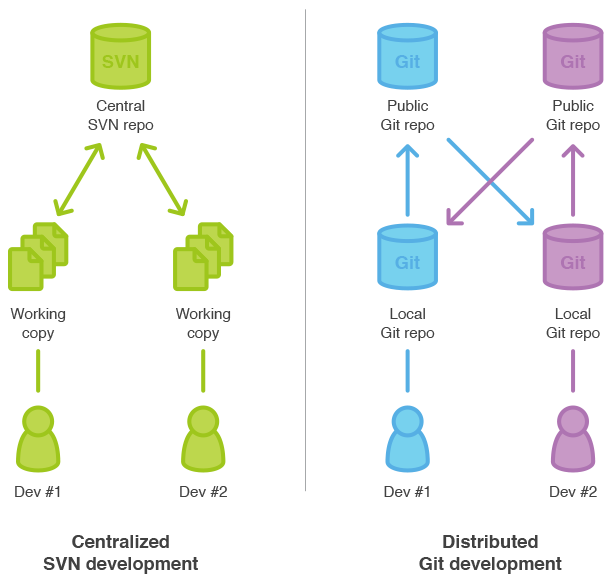
\includegraphics[scale=0.47]{images/gitsvn.png}
    \caption{Różnica w działaniu pomiędzy Git i SVN}
  \end{figure}

  \subsection{RVM}
  \subsection{Narzędzia do testowania}
    \subsubsection{Cucumber}
    \subsubsection{RSpec}
  \subsection{Wykorzystane gemy}
    Gem - jest to paczka napisana w języku Ruby, której zadaniem jest rozszerzenie funkcjonalności aplikacji. Do wyszukiwania najnowszych wersji wykorzystuje się RubyGems.org\footnote{Wyszukiwarka gemów \url{http://rubygems.org}}. W przypadku Ruby on Rails istnieje specjalny plik konfiguracyjny, \emph{Gemfile.rb}, który przechowuje liste wykorzystywanych gemów.

    W naszej aplikacji użyliśmy między innymi:
    \begin{itemize}
      \item \emph{Devise} \\ Zapewnia autoryzacje i autentykacje użytkownika w obrębie aplikacji. Obsługuje logowanie oraz rejestrację wraz z wysyłaniem potwierdzeń na adres mailowy i reset hasła.
      \item \emph{Geocoder} \\ Na podstawie podanego adresu określa współrzędne geograficzne.
      \item \emph{Omniauth-facebook} \\ Wspiera komunikację pomiędzy naszą aplikacją a API Facebook'a.
      \item \emph{i18n} \\ Umożliwia dodawanie tłumaczeń, dzięki czemu aplikacja w łatwy sposób może stać się wielojęzyczną.
    \end{itemize}
  \subsection{Biblioteki JavaScript}
    \begin{itemize}
      \item \emph{jQuery} \\ Biblioteka JavaScript ułatwiająca manipulaję drzewem DOM\footnote{Document Object Model - reprezantacja złożonych dokumentów HTML. \cite{html5_css3}}. Umożliwia tworzenie animacji, wspomaga zarządzanie asynchronicznymi zapytaniami do serwera. Dzięki jej implementacji możliwe jest korzystanie z wielu stworzonych już pluginów.
      \item \emph{Bootstrap Datepicker} \\ Oparta o Bootstrap biblioteka, wyświetlająca na stronie ładny i intuicyjny kalendarz.
      \item \emph{Load Image} \\ Prosta biblioteka umożliwiająca użytkownikowi ładowanie obrazka bezpośrednio na stronie.
      \item Google Maps API
    \end{itemize}
  \subsection{Pozostałe technologie}
    \begin{itemize}
      \item \emph{Bootstrap}
        Framwork CSS, rozwijany przez firmę Twitter. Udostępnia gotowe klasy CSS i rozwiązania JavaScript, dzięki czemu pisanie responsywnych layoutów naitemdzenia mobilne i nie tylko, jest znacznie szybsze i mniej bolesne.
      \item \emph{CoffeScript}
      \item \emph{SASS}
    \end{itemize}
  \subsection{Narzędzia pomocnicze}
    \begin{itemize}
      \item \emph{Sublime Text 3}
      \item \emph{Narzędzia developerskie Google Chrome}
    \end{itemize}
